\section{Flüssigkristalle}
Aggregatszustände:
\begin{itemize}
	\item fest: Moleküle mit 3-dimensionale Fernordnung, anisotrop (richtungsabhängig)
	\item flüssig: ungeordnete Moleküle, isotrop
	\item flüssigkristallin: Moleküle mit 1- oder 2-dimensionaler Fernordnung
\end{itemize}

Flüssigkristalle sind meist nur in einem bestimmten Temperaturbereich flüssigkristallin. Sie bleiben flüssig, haben aber eine höhere Viskosität. Durch die Anisotropie ist eine Trübung oder Farbänderung je nach Blickwinkel möglich. \\

Anwendungen: LCD-Bildschirm, 7-Segment-Anzeige, aufklebbare Temperatursensoren. \\

\subsection{Phasen der Flüssigkristalle}
\begin{figure}[htbp]
	\centering
	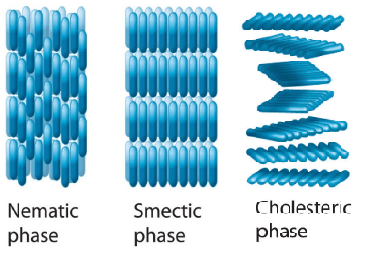
\includegraphics[width=0.5\linewidth]{images/11_Phasen.png}
\end{figure}
\begin{itemize}
	\item nemantische Phase
		\begin{itemize}
			\item 1-dimensionale Ordnung
			\item Moleküle entlang Längsachse ausgerichtet
			\item Molekülenden nicht geordnet
			\item Aneinander Vorbeigleiten möglich
		\end{itemize}
	\item smektische Phase
		\begin{itemize}
			\item 2-dimensionale Ordnung
			\item Moleküle entlang Längsachse ausgerichtet
			\item Molekülenden geordnet $\Rightarrow$ Entstehung von Schichten
			\item Aneinander Vorbeigleiten nicht möglich
			\item SmA: Längsachse in $90^\circ$-Winkel zur Schicht
			\item SmC: Längsachse geneigt zur Schicht
		\end{itemize}
	\item cholestrische Phase
		\begin{itemize}
			\item Schichten mit nematischer Ordnung
			\item jede Schicht um charakteristischen Winkel verdreht (Abstossungskräfte)
			\item Schraubenförmige (helikale) Struktur mit Periodizität im nm-Bereich.
		\end{itemize}
\end{itemize}

\subsection{Atomarer Aufbau}
Flüssigkristalle bestehen aus langen, stabartigen Molekülen mit starren Atomgruppen. 

\begin{figure}[htbp]
	\centering
	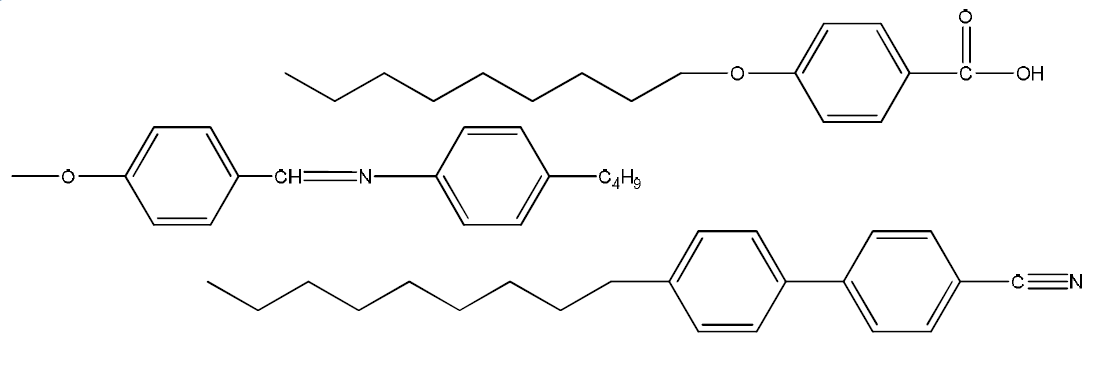
\includegraphics[width=0.8\linewidth]{images/11_Atome.png}
\end{figure}

Zwischenmolekulare Kräfte schränken die Beweglichkeit ein, die Stäbchen richten sich deshalb parallel aus. Da die Atomgruppen meist polar sind, entstehen Dipol-Dipol Kräfte und extern angelegte elektrische Felder können die Moleküle ausrichten (Prinzip des LCD Displays). 